\subsection{Conversion from Depth Image to Feature Image}\label{sec:feature_images}

The conversion of depth images to feature images needs to result in a single scalar value because all keypoint detectors work on a single signal channel.
Every feature image is calculated on range data in floating point format, potentially requiring the preprocessing step presented in Section~\ref{sec:range_depth_conversion}.
The representation change from integer to floating point data does no further processing than simple type conversion.

This section introduces and develops multiple potential feature images that were considered during this thesis.
Conversions for images of the \emph{Synthetic} scene (Section~\ref{sec:dataset_synthetic}) containing different primitive geometric structures serve as examples for the visual appeal of each feature image type.

\subsubsection{Bearing-Angle Image}

\begin{figure}[H]
    \centering
    \scalebox{0.9}{%
    

\tikzset{every picture/.style={line width=0.75pt}} %set default line width to 0.75pt        

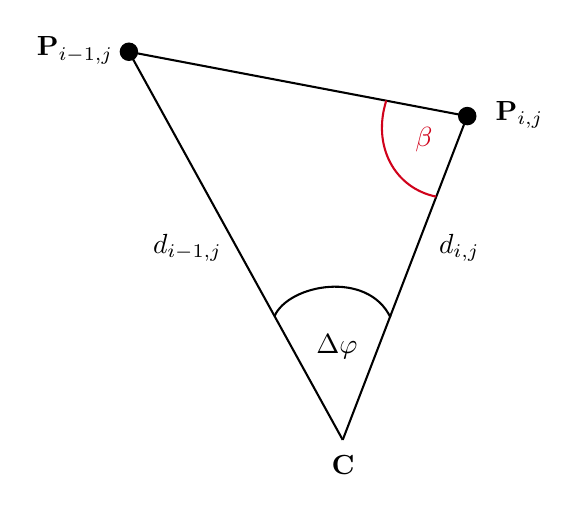
\begin{tikzpicture}[x=0.75pt,y=0.75pt,yscale=-1,xscale=1]
%uncomment if require: \path (0,228); %set diagram left start at 0, and has height of 228

%Straight Lines [id:da05017383740499093] 
\draw    (42.83,15.67) -- (145.83,202.67) ;
%Straight Lines [id:da6895513561877372] 
\draw    (205.83,46.67) -- (145.83,202.67) ;
%Curve Lines [id:da10253757735662583] 
\draw [color={rgb, 255:red, 0; green, 0; blue, 0 }  ,draw opacity=1 ]   (113,143) .. controls (119.83,127.67) and (157.83,120.67) .. (168.83,143.67) ;
%Straight Lines [id:da3851492122035306] 
\draw    (42.83,15.67) -- (205.83,46.67) ;
%Curve Lines [id:da7052636563383052] 
\draw [color={rgb, 255:red, 208; green, 2; blue, 27 }  ,draw opacity=1 ]   (166.83,39.17) .. controls (159.83,61.17) and (170.9,81.48) .. (190.9,85.48) ;
%Shape: Circle [id:dp08101382020617043] 
\draw  [fill={rgb, 255:red, 0; green, 0; blue, 0 }  ,fill opacity=1 ] (201.88,46.67) .. controls (201.88,44.49) and (203.65,42.72) .. (205.83,42.72) .. controls (208.01,42.72) and (209.78,44.49) .. (209.78,46.67) .. controls (209.78,48.85) and (208.01,50.62) .. (205.83,50.62) .. controls (203.65,50.62) and (201.88,48.85) .. (201.88,46.67) -- cycle ;
%Shape: Circle [id:dp7397482298206297] 
\draw  [fill={rgb, 255:red, 0; green, 0; blue, 0 }  ,fill opacity=1 ] (38.88,15.67) .. controls (38.88,13.49) and (40.65,11.72) .. (42.83,11.72) .. controls (45.01,11.72) and (46.78,13.49) .. (46.78,15.67) .. controls (46.78,17.85) and (45.01,19.62) .. (42.83,19.62) .. controls (40.65,19.62) and (38.88,17.85) .. (38.88,15.67) -- cycle ;

% Text Node
\draw (143,158) node  [color={rgb, 255:red, 0; green, 0; blue, 0 }  ,opacity=1 ] [align=left] {$\displaystyle \Delta $$\displaystyle \varphi $};
% Text Node
\draw (185,58) node  [color={rgb, 255:red, 208; green, 2; blue, 27 }  ,opacity=1 ] [align=left] {$\displaystyle \beta $};
% Text Node
\draw (202,110) node   [align=left] {$\displaystyle d_{i,j}$};
% Text Node
\draw (71,110) node   [align=left] {$\displaystyle d_{i-1,j}$};
% Text Node
\draw (231,46) node   [align=left] {$\displaystyle \mathbf{P}_{i,j}$};
% Text Node
\draw (16.83,15) node   [align=left] {$\displaystyle \mathbf{P}_{i-1,j}$};
% Text Node
\draw (146,215) node   [align=left] {$\displaystyle \mathbf{C}$};


\end{tikzpicture}

%
    }
    \caption[Schematic representation of \glspl{bearing-angle}]{\emph{Schematic representation of \glspl{bearing-angle}.} This figure shows the relationship of the light rays that form the \gls{bearing-angle} $\beta$.}\label{fig:bearing_angle}
\end{figure}

Scaramuzza\cite{scaramuzza_iros2007} proposes \Glspl{bearing-angle-image} that assigns each pixel the angle $\beta$ as Figure~\ref{fig:bearing_angle} demonstrates.
This angle is spanned by the two idealized lightrays for pixels of the range image.
The neighbourhood relationship between pixels can be choosen arbitrarily resulting in four \Glspl{bearing-angle-image}, horizontal, vertical, diagonal and antidiagonal.
The second variable is the direction the angle is calculted, e.g.~for horizontal images it can be calculated from left-to-right or right-to-left.
This does not exhibit new information, because the angle of the other direction is immediatly known from the fact that the sum of the angles is $180\degree$.
Nontheless, the direction must be defined to obtain stable results.

The formula for the \gls{bearing-angle} $\beta$ is derived with the cosine theorem.
Note, that both Scaramuzza\cite{scaramuzza_iros2007} and Lin\cite{lin_easp2017} have typos in the formulae they provided.
A full derivation for the correct equation is provided in Appendix~\ref{sec:bearing_derivation}.
For the horizontal left-to-right calculation the formula is as follows.
\begin{equation}\label{eq:bearing-angle}
    \beta = \arccos%
            \frac{d_{i,j} - d_{i-1,j} \cos \Delta\varphi}%
                 {\sqrt{d_{i,j}^2 + d_{i-1,j}^2 - 2 d_{i,j} d_{i-1,j} \cos \Delta\varphi}}
\end{equation}
The angular resolution $\Delta\varphi$ between two pixels of the depth image depends on the camera model in use.
The pinhole model's angular resolution changes between pixel pairs, equirectangular image have a constant resolution.
In general, the angle $\Delta\varphi$ can be calculated with the spherical coordinates $\mathbf{P_{\mathcal{S},1}}, \mathbf{P_{\mathcal{S},2}}$ of the pixel pair $\mathbf{p_1}, \mathbf{p_2}$.
Optimized versions for the specific camera model are possible in real world applications.
\begin{equation}
\begin{aligned}
    \abs{\vec{P_{\mathcal{S},1}}} &= \abs{\vec{P_{\mathcal{S},2}}} = 1 \implies \vec{P_{\mathcal{S},1}} \cdot \vec{P_{\mathcal{S},2}} = \cos \Delta\varphi \\
    \Delta\varphi &= \arccos \vec{P_{\mathcal{S},1}} \cdot \vec{P_{\mathcal{S},2}}
\end{aligned}
\end{equation}

The \Gls{bearing-angle} is in the range $\beta \in (0, \pi)~rad$.
Linear scaling of the angle to the color depth of the target image results in a grayscale image suitable for feature extraction.
A general scaling function for an \emph{unsigned 8bit} image and arbitrary angle range follows here.
This formulation can be used for different color depths and other potential angle calculations that result in different boundary conditions.
\begin{equation}
\begin{aligned}
\label{eq:linear_scaling}
    \beta_{min} &= 0 ~& c_{min} &= 0 \\
    \beta_{max} &= \pi ~& c_{max} &= 255 \\
    \beta_{scaled} &= \floor*{c_{min} + \beta \frac{c_{max} - c_{min}}{\beta_{max} - \beta_{min}}}
\end{aligned}
\end{equation}

\subsubsection*{Characteristics}

\begin{figure}[H]
    \begin{subfigure}[t]{0.32\textwidth}
        
\includegraphics[width=\linewidth]{chapter04/img/bearing-diag-0001.png}
    \end{subfigure}
    \begin{subfigure}[t]{0.32\textwidth}
        
\includegraphics[width=\linewidth]{chapter04/img/bearing-diag-0030.png}
    \end{subfigure}
    \begin{subfigure}[t]{0.32\textwidth}
        
\includegraphics[width=\linewidth]{chapter04/img/bearing-diag-0210.png}
    \end{subfigure}
    \caption[\gls{bearing-angle-image} characteristics]{\emph{\gls{bearing-angle-image} characteristics.} The \gls{bearing-angle-image} is not invariant to rotation and viewpoint changes. This property limits its applicability for automatic registration of bigger discontinues changes of the camera pose. Each depth image was converted with the diagonal (top-left-to-bottom-right direction) implementation of the \gls{bearing-angle} formula.}\label{fig:bearing_characteristics}
\end{figure}
A deeper understanding of the \gls{bearing-angle-image} helps to understand advantages and disadvantages for its usage.
Figure~\ref{fig:bearing_characteristics} demonstrates the visual changes of a synthetic scene under certain camera transformations.

The most notable property is the lack of rotation invariance.
This follows directly from the definition of the \gls{bearing-angle}.
A triangle is build by a predefined pixel relationship.
Calculating the \gls{bearing-angle} from multiple directions could lead to some rotation stability, because rotations of $45\degree$ corresponds to a different direction of pixel neighbourhood.
\begin{figure}[H]
    \centering
    

\tikzset{every picture/.style={line width=0.75pt}} %set default line width to 0.75pt        

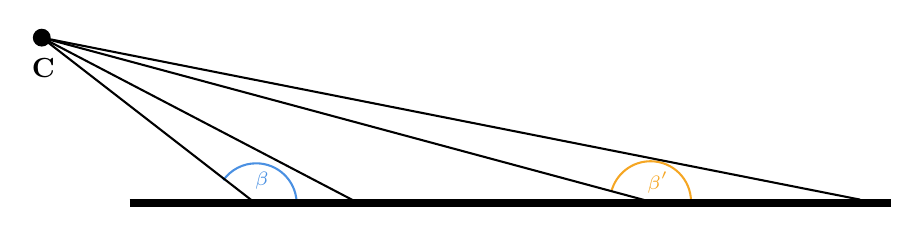
\begin{tikzpicture}[x=0.75pt,y=0.75pt,yscale=-1,xscale=1]
%uncomment if require: \path (0,111); %set diagram left start at 0, and has height of 111

%Shape: Arc [id:dp6607157958124017] 
\draw  [draw opacity=0] (294.74,88.39) .. controls (296.93,80.02) and (304.55,73.85) .. (313.6,73.85) .. controls (324.37,73.85) and (333.1,82.58) .. (333.1,93.35) -- (313.6,93.35) -- cycle ; \draw  [color={rgb, 255:red, 245; green, 166; blue, 35 }  ,draw opacity=1 ] (294.74,88.39) .. controls (296.93,80.02) and (304.55,73.85) .. (313.6,73.85) .. controls (324.37,73.85) and (333.1,82.58) .. (333.1,93.35) ;
%Shape: Arc [id:dp6461315771728425] 
\draw  [draw opacity=0] (107.76,82.98) .. controls (111.29,78.06) and (117.07,74.85) .. (123.6,74.85) .. controls (134.06,74.85) and (142.59,83.08) .. (143.08,93.42) -- (123.6,94.35) -- cycle ; \draw  [color={rgb, 255:red, 74; green, 144; blue, 226 }  ,draw opacity=1 ] (107.76,82.98) .. controls (111.29,78.06) and (117.07,74.85) .. (123.6,74.85) .. controls (134.06,74.85) and (142.59,83.08) .. (143.08,93.42) ;
%Straight Lines [id:da7912546873109455] 
\draw [line width=3]    (62.6,94) -- (429.6,94) ;
%Shape: Circle [id:dp6585955324129855] 
\draw  [draw opacity=0][fill={rgb, 255:red, 0; green, 0; blue, 0 }  ,fill opacity=1 ] (16,14.3) .. controls (16,11.93) and (17.93,10) .. (20.3,10) .. controls (22.67,10) and (24.6,11.93) .. (24.6,14.3) .. controls (24.6,16.67) and (22.67,18.6) .. (20.3,18.6) .. controls (17.93,18.6) and (16,16.67) .. (16,14.3) -- cycle ;
%Straight Lines [id:da6943190688257042] 
\draw    (20.3,14.3) -- (123.6,94.35) ;
%Straight Lines [id:da2008172675955413] 
\draw    (20.3,14.3) -- (171.6,93.35) ;
%Straight Lines [id:da41493445776640725] 
\draw    (20.3,14.3) -- (313.6,93.35) ;
%Straight Lines [id:da4646477074321278] 
\draw    (20.3,14.3) -- (414.6,92.35) ;

% Text Node
\draw (14,23) node [anchor=north west][inner sep=0.75pt]   [align=left] {$\displaystyle \mathbf{C}$};
% Text Node
\draw (121.6,77.35) node [anchor=north west][inner sep=0.75pt]  [font=\scriptsize,color={rgb, 255:red, 74; green, 144; blue, 226 }  ,opacity=1 ] [align=left] {$\displaystyle \beta $};
% Text Node
\draw (310.6,77.35) node [anchor=north west][inner sep=0.75pt]  [font=\scriptsize,color={rgb, 255:red, 245; green, 166; blue, 35 }  ,opacity=1 ] [align=left] {$\displaystyle \beta '$};


\end{tikzpicture}

%
    \caption[Two \glspl{bearing-angle} for the same ground plane]{\emph{Two \glspl{bearing-angle} for the same ground plane.} Different shadings of plane surfaces depend on the perspective projection and the distance from the camera center $C$ to the surface.}\label{fig:bearing_angle_shading}
\end{figure}
The second apparent aspect is the change in shading for example the flat ground, but other surfaces as well.
This effect is due to the perspective transformation and the distance of a point to the camera, as Figure~\ref{fig:bearing_angle_shading} demonstrates.
Round objects, like spheres, experience no visual change in shading.
The triangles of the lightrays are invariant to camera transformation for such objects.

\subsubsection{Multi-Directional Bearing Angle}

The \emph{Multi-Directional \gls{bearing-angle-image}} attempts to overcome the limitation of missing rotation invariance for the classical \gls{bearing-angle-image}.
Instead of just one angle in one direction, the two adjacent triangle are analyzed together.
Figure~\ref{fig:max-curve} shows how the triangles are related.
Both angles $\beta$ and $\gamma$ are calculated with equation~\ref{eq:bearing-angle}, for $\gamma$ the values of $d_{i,j}$ and $d_{i-1,j}$ just need to be swapped.
\begin{figure}
    

\tikzset{every picture/.style={line width=0.75pt}} %set default line width to 0.75pt        

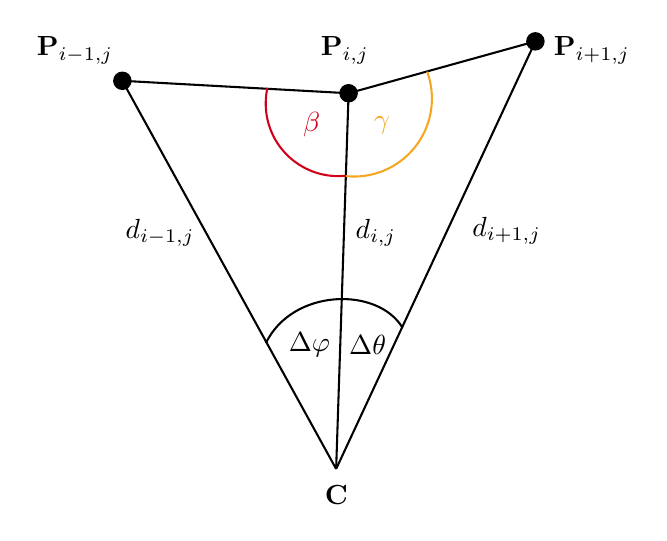
\begin{tikzpicture}[x=0.75pt,y=0.75pt,yscale=-1,xscale=1]
%uncomment if require: \path (0,252); %set diagram left start at 0, and has height of 252

%Straight Lines [id:da05017383740499093] 
\draw    (46.83,26.67) -- (149.83,213.67) ;
%Straight Lines [id:da6895513561877372] 
\draw    (155.83,32.67) -- (149.83,213.67) ;
%Curve Lines [id:da10253757735662583] 
\draw [color={rgb, 255:red, 0; green, 0; blue, 0 }  ,draw opacity=1 ]   (116,153) .. controls (128.83,126.67) and (169.83,125.67) .. (181.83,145.67) ;
%Straight Lines [id:da3851492122035306] 
\draw    (46.83,26.67) -- (155.83,32.67) ;
%Shape: Circle [id:dp08101382020617043] 
\draw  [fill={rgb, 255:red, 0; green, 0; blue, 0 }  ,fill opacity=1 ] (151.88,32.67) .. controls (151.88,30.49) and (153.65,28.72) .. (155.83,28.72) .. controls (158.01,28.72) and (159.78,30.49) .. (159.78,32.67) .. controls (159.78,34.85) and (158.01,36.62) .. (155.83,36.62) .. controls (153.65,36.62) and (151.88,34.85) .. (151.88,32.67) -- cycle ;
%Shape: Circle [id:dp7397482298206297] 
\draw  [fill={rgb, 255:red, 0; green, 0; blue, 0 }  ,fill opacity=1 ] (42.88,26.67) .. controls (42.88,24.49) and (44.65,22.72) .. (46.83,22.72) .. controls (49.01,22.72) and (50.78,24.49) .. (50.78,26.67) .. controls (50.78,28.85) and (49.01,30.62) .. (46.83,30.62) .. controls (44.65,30.62) and (42.88,28.85) .. (42.88,26.67) -- cycle ;
%Shape: Circle [id:dp7936487176657823] 
\draw  [fill={rgb, 255:red, 0; green, 0; blue, 0 }  ,fill opacity=1 ] (241.88,7.67) .. controls (241.88,5.49) and (243.65,3.72) .. (245.83,3.72) .. controls (248.01,3.72) and (249.78,5.49) .. (249.78,7.67) .. controls (249.78,9.85) and (248.01,11.62) .. (245.83,11.62) .. controls (243.65,11.62) and (241.88,9.85) .. (241.88,7.67) -- cycle ;
%Straight Lines [id:da7225304487809803] 
\draw    (245.83,7.67) -- (149.83,213.67) ;
%Straight Lines [id:da15289701870660388] 
\draw    (155.83,32.67) -- (245.83,7.67) ;
%Shape: Arc [id:dp845909277560968] 
\draw  [draw opacity=0] (154.29,72.43) .. controls (153.16,72.54) and (152.02,72.6) .. (150.87,72.6) .. controls (131.56,72.6) and (115.9,56.94) .. (115.9,37.63) .. controls (115.9,35.08) and (116.17,32.59) .. (116.69,30.19) -- (150.87,37.63) -- cycle ; \draw  [color={rgb, 255:red, 208; green, 2; blue, 27 }  ,draw opacity=1 ] (154.29,72.43) .. controls (153.16,72.54) and (152.02,72.6) .. (150.87,72.6) .. controls (131.56,72.6) and (115.9,56.94) .. (115.9,37.63) .. controls (115.9,35.08) and (116.17,32.59) .. (116.69,30.19) ;
%Shape: Arc [id:dp15343497156889918] 
\draw  [draw opacity=0] (193.67,22.29) .. controls (195.16,26.33) and (195.97,30.7) .. (195.97,35.25) .. controls (195.97,55.99) and (179.15,72.8) .. (158.42,72.8) .. controls (157.06,72.8) and (155.72,72.73) .. (154.4,72.59) -- (158.42,35.25) -- cycle ; \draw  [color={rgb, 255:red, 245; green, 166; blue, 35 }  ,draw opacity=1 ] (193.67,22.29) .. controls (195.16,26.33) and (195.97,30.7) .. (195.97,35.25) .. controls (195.97,55.99) and (179.15,72.8) .. (158.42,72.8) .. controls (157.06,72.8) and (155.72,72.73) .. (154.4,72.59) ;

% Text Node
\draw (137,154) node  [color={rgb, 255:red, 0; green, 0; blue, 0 }  ,opacity=1 ] [align=left] {$\displaystyle \Delta $$\displaystyle \varphi $};
% Text Node
\draw (138,48) node  [color={rgb, 255:red, 208; green, 2; blue, 27 }  ,opacity=1 ] [align=left] {$\displaystyle \beta $};
% Text Node
\draw (169,100) node   [align=left] {$\displaystyle d_{i,j}$};
% Text Node
\draw (65,100) node   [align=left] {$\displaystyle d_{i-1,j}$};
% Text Node
\draw (154,12) node   [align=left] {$\displaystyle \mathbf{P}_{i,j}$};
% Text Node
\draw (150,226) node   [align=left] {$\displaystyle \mathbf{C}$};
% Text Node
\draw (232,99) node   [align=left] {$\displaystyle d_{i+1,j}$};
% Text Node
\draw (172,48) node   [align=left] {$\displaystyle \textcolor[rgb]{0.96,0.65,0.14}{\gamma }$};
% Text Node
\draw (165,154) node  [color={rgb, 255:red, 0; green, 0; blue, 0 }  ,opacity=1 ] [align=left] {$\displaystyle \Delta $$\displaystyle \theta $};
% Text Node
\draw (273,12) node   [align=left] {$\displaystyle \mathbf{P}_{i+1,j}$};
% Text Node
\draw (24,12) node   [align=left] {$\displaystyle \mathbf{P}_{i-1,j}$};


\end{tikzpicture}


    \caption[Schematic Representation of the Multi-Directional \gls{bearing-angle-image}]{The Multi-Directional \gls{bearing-angle-image} composes two \Glspl{bearing-angle} in vertical, horizontal, diagonal and antidiagonal direction. The maximum angle is then selected as pixel value.}\label{fig:max-curve}
\end{figure}
Both angles are added together, resulting in the angle of an edge at this position.
\begin{equation}
    \mathcal{B} = \beta + \gamma
\end{equation}
This calculation is again only in one direction and not rotation invariant but already symmetrical.
The value $B$ can be defined for diagonal, antidiagonal, horizontal and vertical sampling of the image.
The final step for rotation invariance is the reduction of these four values to its maximum.
\begin{align}
    \mathcal{B} &= \max{\{\mathcal{B}_{diagonal}, \mathcal{B}_{antidiagonal}, \mathcal{B}_{horizontal}, \mathcal{B}_{vertical}\}}
\end{align}
The converted images in Figure~\ref{fig:max-curve-images} show the same scene and positions as for the \gls{bearing-angle-image}.
\begin{figure}[H]
    \begin{subfigure}[t]{0.32\textwidth}
        
\includegraphics[width=\linewidth]{chapter04/img/max-0001.png}
    \end{subfigure}
    \begin{subfigure}[t]{0.32\textwidth}
        
\includegraphics[width=\linewidth]{chapter04/img/max-0030.png}
    \end{subfigure}
    \begin{subfigure}[t]{0.32\textwidth}
        
\includegraphics[width=\linewidth]{chapter04/img/max-0210.png}
    \end{subfigure}
    \caption{The subfigures show the same camera positions as the \gls{bearing-angle} and demonstrates the rotation invariance. Each edge in the geometry forms a visible white line. No other textures exist.}\label{fig:max-curve-images}
\end{figure}
The goal of rotational invariance is achieved, unfortunatly the image lacks texture and contrast.
Qualitative tests with common feature detectors yielded weak keypoint responses.
Therefore, this approach received no further attention.

\subsubsection{Curvature Image}

Differential geometry provides a scalar quantity assignable to each point of a one-dimensional differntiable function, the \emph{\gls{curvature}} $\kappa$\cite[p. 10]{Kuhnel2008}.
This concept can be generalized to higher dimensions and two common \glspl{curvature} exist for surfaces in three-dimensional space, \emph{\gls{gaussian-curvature}} and \emph{\gls{mean-curvature}}.
\begin{figure}[t]
    \begin{subfigure}[t]{0.48\textwidth}
        \centering
        \scalebox{0.85}{%
        \begin{tikzpicture}
\begin{axis}[xmin=-0.7,
             xmax=0.7,
             ymin=-0.1,
             ymax=1.1,
             samples=200,
             axis line style={draw=none},
             tick style={draw=none},
             xticklabels={\empty},
             yticklabels={\empty},
             grid=major,
             plot box ratio={2 1},
             axis equal]
    \draw[plotorange, line width=1.3pt] (axis cs:0,0.5) circle [radius=50];
    \addplot[plotblue, line width=1.5pt] {x*x};
    \coordinate (C) at (axis cs:{0.0,0.5});
    \coordinate (O) at (axis cs:{0.0,0.0});
    \coordinate (L) at (axis cs:{0.1,0.25});
    \node at (L) {$\mathbf{r}$};
    \node[label={90:{$\mathbf{C}$}},circle,fill,inner sep=1pt] at (C) {};
    \draw[thick,-](C)--(O);
\end{axis}
\end{tikzpicture}

        }
        \caption{The \gls{curvature} of a line at a specific point is defined by its osculating circle.}\label{fig:osculating_circle}
    \end{subfigure}\hfill%
    \begin{subfigure}[t]{0.48\textwidth}
        \centering
        \scalebox{0.85}{%
        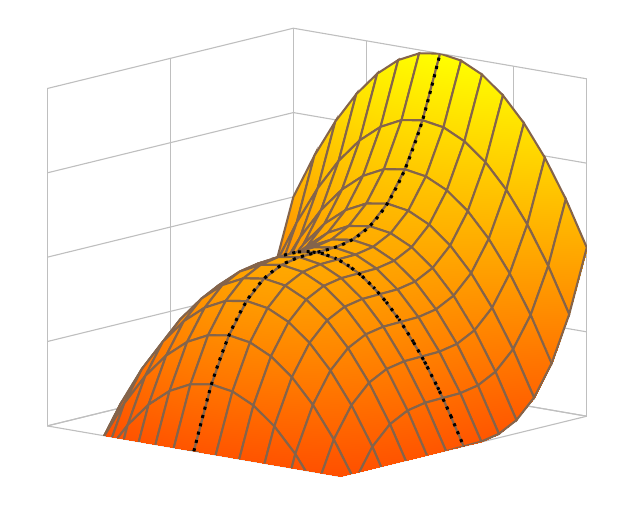
\begin{tikzpicture}
\begin{axis}[xmin=-1.0,xmax=1.0,
             ymin=-1.0,ymax=1.0,
             zmin=-1.0,zmax=1.0,
             grid=major,
             axis line style={draw=none},
             tick style={draw=none},
             view={310}{35},
             xticklabels={\empty},
             yticklabels={\empty},
             zticklabels={\empty},
             plot box ratio={1 1 3},
             colormap/redyellow]
\newcommand\func[2]{#1^3 - #2^2}
\definecolor{darkorange}{HTML}{84644B}

    \addplot3[surf,
              shader=faceted interp,
              faceted color={darkorange},
              samples=15,
              domain=-1:1,
              y domain=-1:1] {\func{x}{y}};

    % plot curve for x direction
    \addplot3[samples=15,
              domain=-1:1,
              samples y=1,
              dotted,
              black,
              line width=1.1pt,
              smooth] (x, 0, \func{x}{0});
    % plot curve for y direction
    \addplot3[samples=15,
              domain=-1:1,
              y domain=-1:0.22,
              dotted,
              black,
              line width=1.1pt,
              smooth] (0, y, \func{0}{y});
\end{axis}
\end{tikzpicture}

        }
        \caption{The principal curvatures are the maximum and minimum \glspl{curvature} in all directions.}\label{fig:curvature_surface}
    \end{subfigure}
    \caption[Curvature of curves and surfaces]{\emph{Curvature of curves and surfaces.} The \gls{curvature} of a curve is defined through its osculating circle. This simple definition is not possible for surfaces in three dimensions. Analyzing all directions, each point on the surface does have a minimum and maximum \gls{curvature} --- the \emph{principal curvatures}.}
\end{figure}
A straight line has no \gls{curvature}, hence $\kappa = 0$.
The \gls{curvature} of a circle is defined is the inverse of its radius
\begin{equation}
    \kappa_{circle} = \frac{1}{r}\text{.}
\end{equation}
Any point's \gls{curvature} on a one-dimensional, twice differentiable function is defined as the \gls{curvature} of its osculating circle, visualized in Figure~\ref{fig:osculating_circle}.
The \gls{curvature} of any point of a surface in three-dimensional space is ambigous, because it has infinite many curves crossing through this point.
But a maximum and minimum \gls{curvature} exist, the \emph{principal curvatures} $k_1$ and $k_2$.
Figure~\ref{fig:curvature_surface} visualizes the directions of the minimum and maximum \gls{curvature} of a surface in three-dimensional space as dotted black lines.
The \emph{\Gls{gaussian-curvature}} $\mathcal{K}$ is defined as the product
\begin{equation}
    \mathcal{K} = k_1 k_2
\end{equation}
and the \emph{\gls{mean-curvature}} $\mathcal{H}$ as the mean
\begin{equation}
    \mathcal{H} = \frac{1}{2} (k_1 k_2)
\end{equation}
of the principal curvatures.

Both quantities can be calculated differently, as the \gls{curvature} is related to the derivates of a function.
Let $f(u, v)$ be a two-dimensional function representing the depth image and $f_u$, $f_v$, $f_{uu}$ and $f_{vv}$ its partial derivatives.
Then the \gls{gaussian-curvature} and \gls{mean-curvature} are computed with:
\begin{equation}
\begin{aligned}
    \mathcal{K} &= \frac{f_{uu} f_{vv} - f_{uv}^2}{{(1 + f_u^2 + f_v^2)}^2}\text{,} \\
    \mathcal{H} &= \frac{{(1 + f_{v}^2)} f_{uu} - 2 f_u f_v f_{uv} + {(1 + f_u^2)} f_{vv}}{2 \sqrt{1 + f_u^2 + f_v^2}^3}\text{.}
\end{aligned}
\end{equation}
The central differential quotients approximate the first and second derivatives with $\mathcal{O}(\Delta x^2)$ accuracy:
\begin{equation}
\begin{aligned}
    f_{x} &= \frac{y_{i+1} - y_{i-1}}{2 \Delta x} \\
    f_{xx} &= \frac{y_{i+1} + y_{i-1} - 2 y_{i}}{{\Delta x}^2}\text{.}
\end{aligned}
\end{equation}

\begin{figure}[tb]
    \begin{subfigure}[t]{0.32\textwidth}
        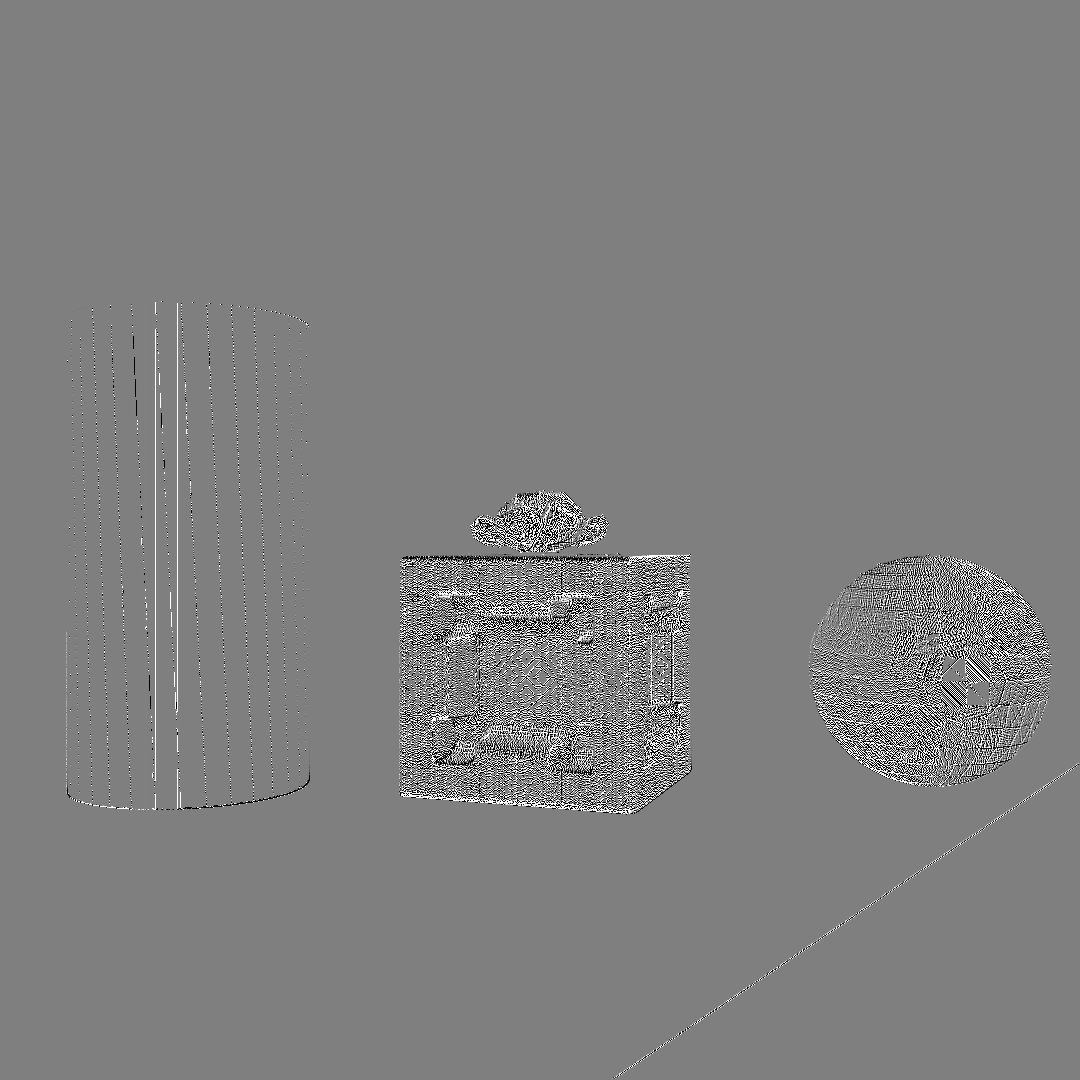
\includegraphics[width=\linewidth]{chapter04/img/mean-0001.png}
    \end{subfigure}
    \begin{subfigure}[t]{0.32\textwidth}
        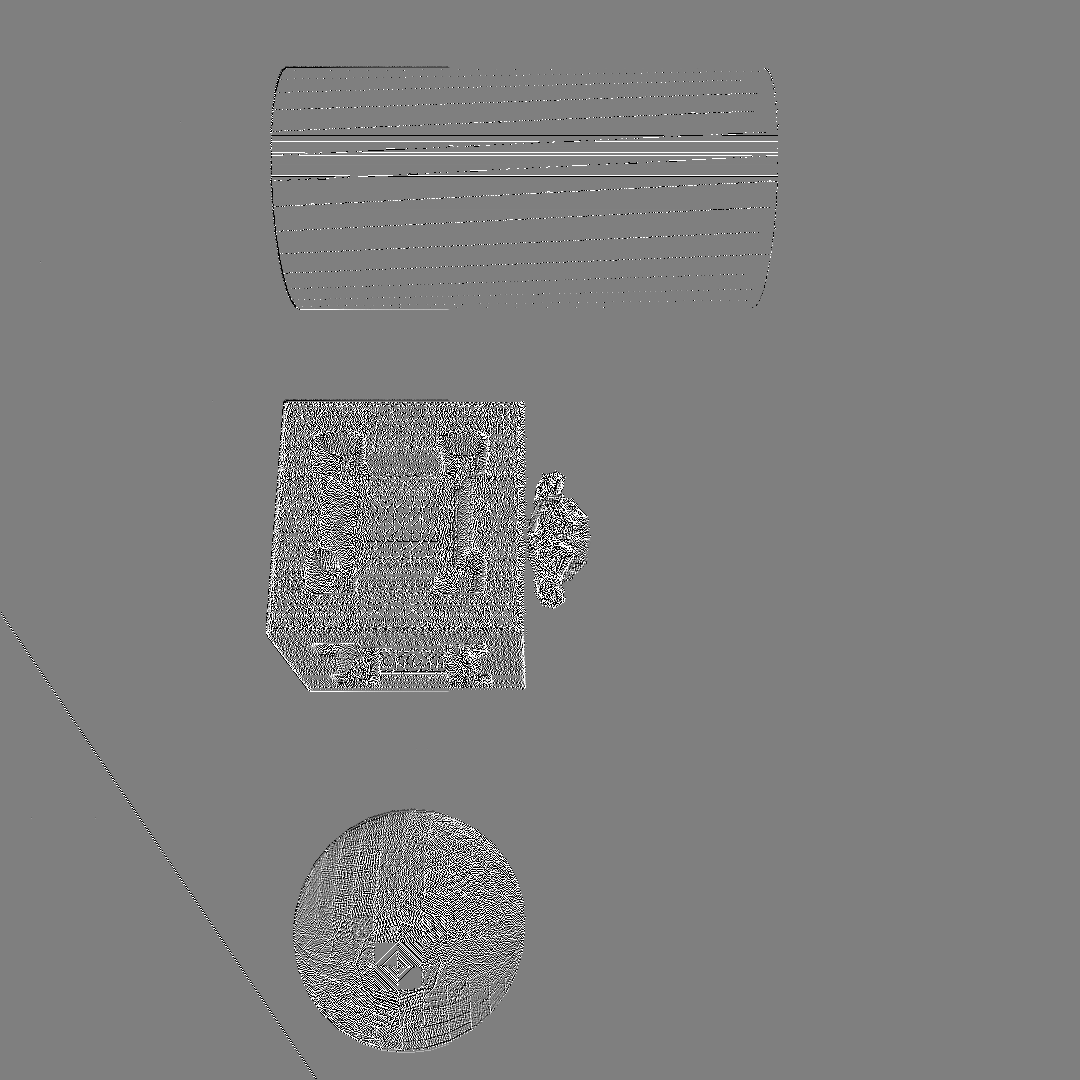
\includegraphics[width=\linewidth]{chapter04/img/mean-0030.png}
    \end{subfigure}
    \begin{subfigure}[t]{0.32\textwidth}
        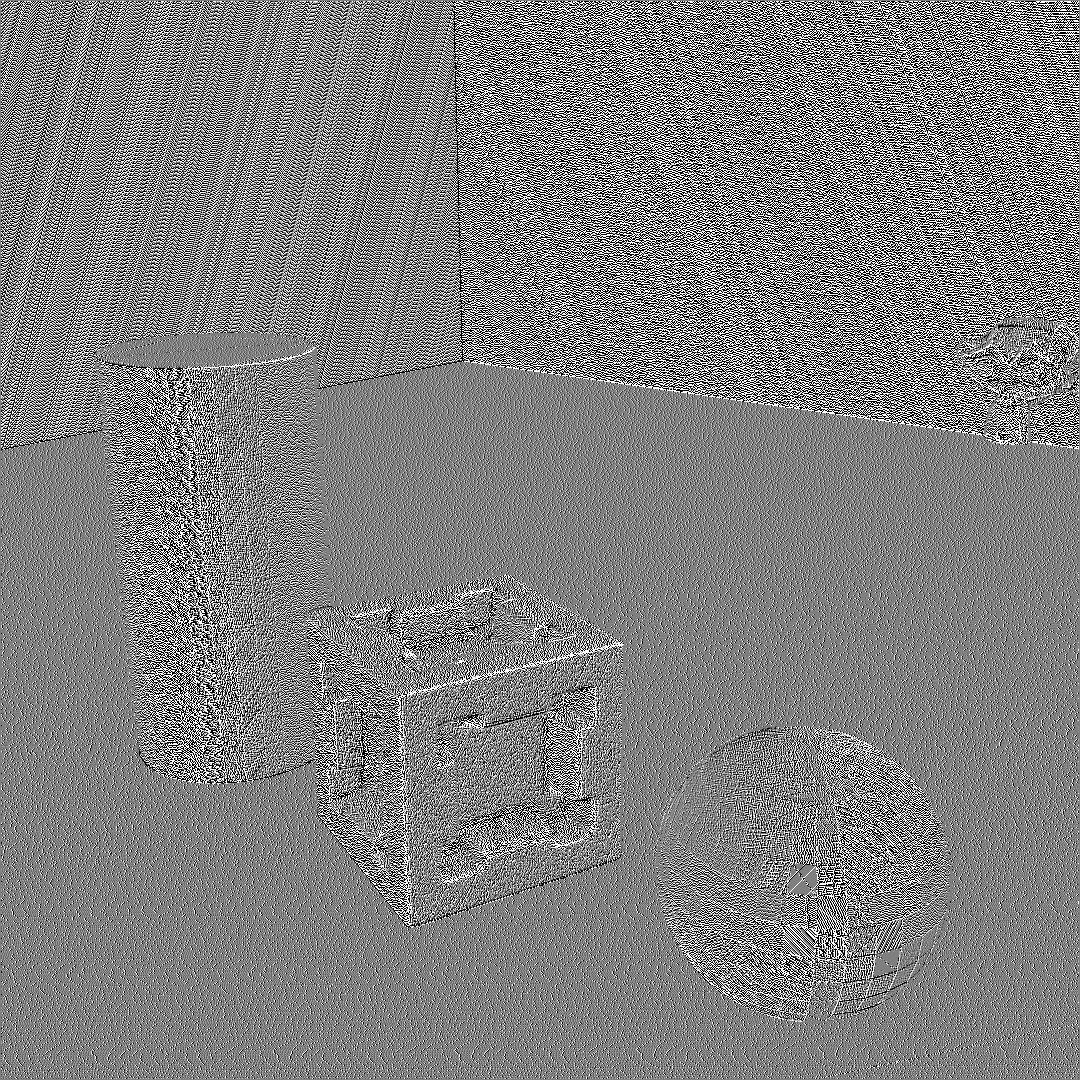
\includegraphics[width=\linewidth]{chapter04/img/mean-0210.png}
    \end{subfigure}
    \caption[\Gls{mean-curvature} in the \emph{Synthetic} scene]{\emph{\Gls{mean-curvature} in the Synthetic scene.} The \gls{mean-curvature} feature image for the same synthetic scene are similar to Multi-Directional \Glspl{bearing-angle-image}, making them a second non-promising option.}\label{fig:mean-curvature}
\end{figure}
The result of the \gls{mean-curvature} conversion in Figure~\ref{fig:mean-curvature} is similar to the Multi-Directional \gls{bearing-angle-image}.
The \gls{mean-curvature} is rotation invariant but the result is already very unstable to the noise induced by integer precision depth images.
Figure~\ref{fig:gaussian-curvature} shows the images for the \gls{gaussian-curvature}.
It is even more prone to noise in the input and suffers from the same range issue.

Both the \gls{mean-curvature} and \gls{gaussian-curvature} are unbound and result in any real number.
Simple scaling between the computed minimum and maximum value is unstable between images and results in completly gray images as these quantities have noticable outliers.
As solution for this problem the computed values are clamped to a predefined range, for example $\mathcal{H},\mathcal{K} \in (-20, 20)$ and then scaled to the desired image depth of the feature image.
\begin{figure}[tb]
    \begin{subfigure}[t]{0.32\textwidth}
        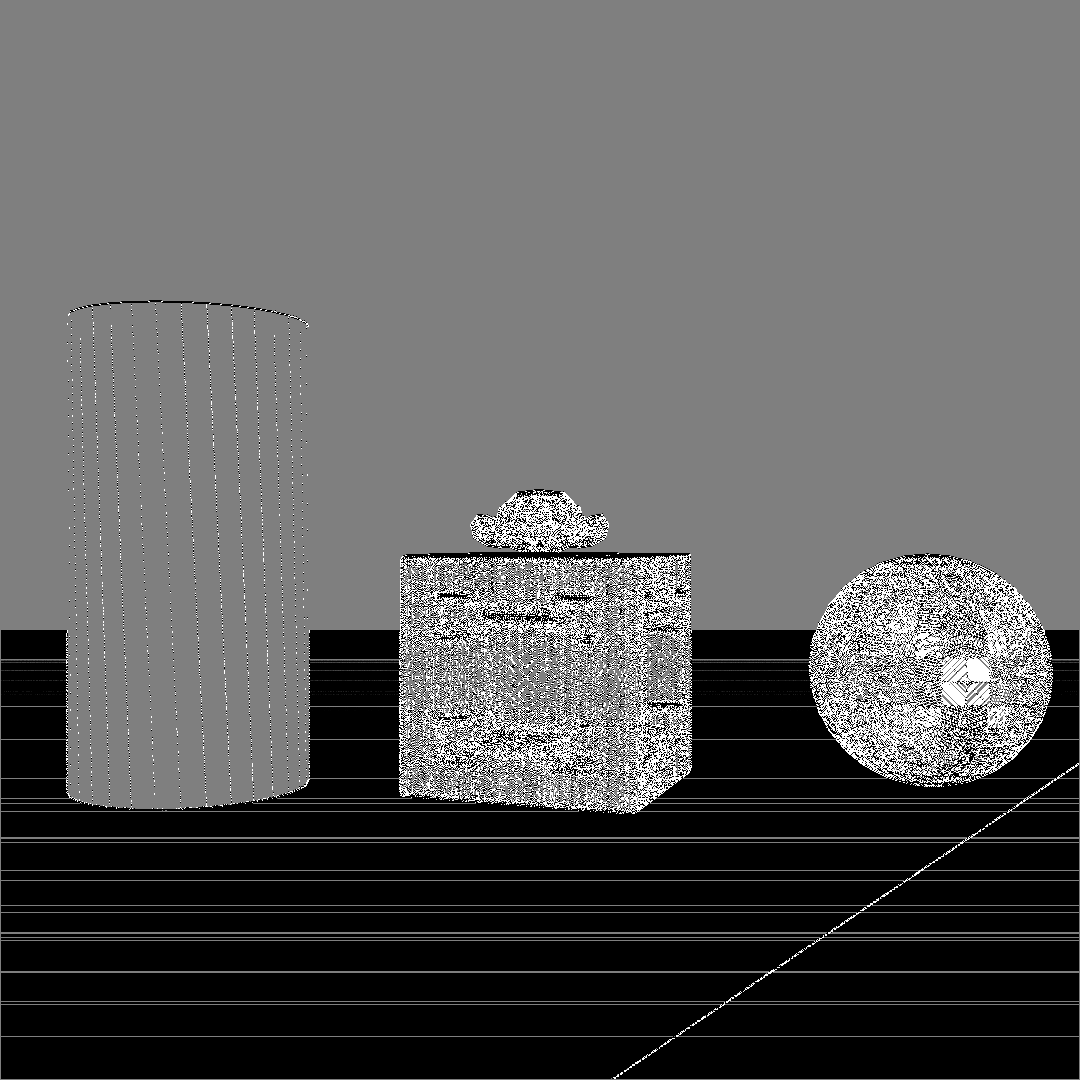
\includegraphics[width=\linewidth]{chapter04/img/gauss-0001.png}
    \end{subfigure}
    \begin{subfigure}[t]{0.32\textwidth}
        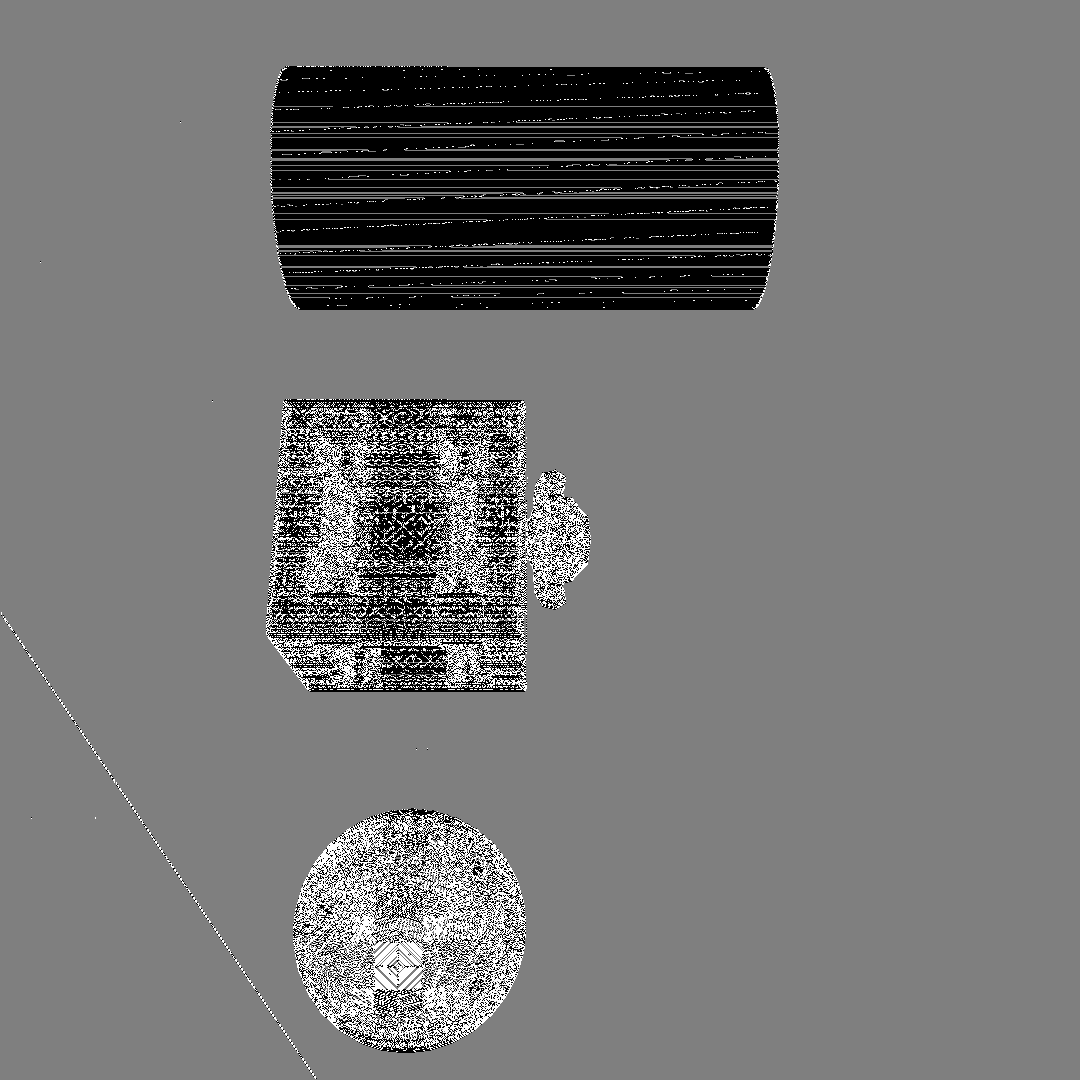
\includegraphics[width=\linewidth]{chapter04/img/gauss-0030.png}
    \end{subfigure}
    \begin{subfigure}[t]{0.32\textwidth}
        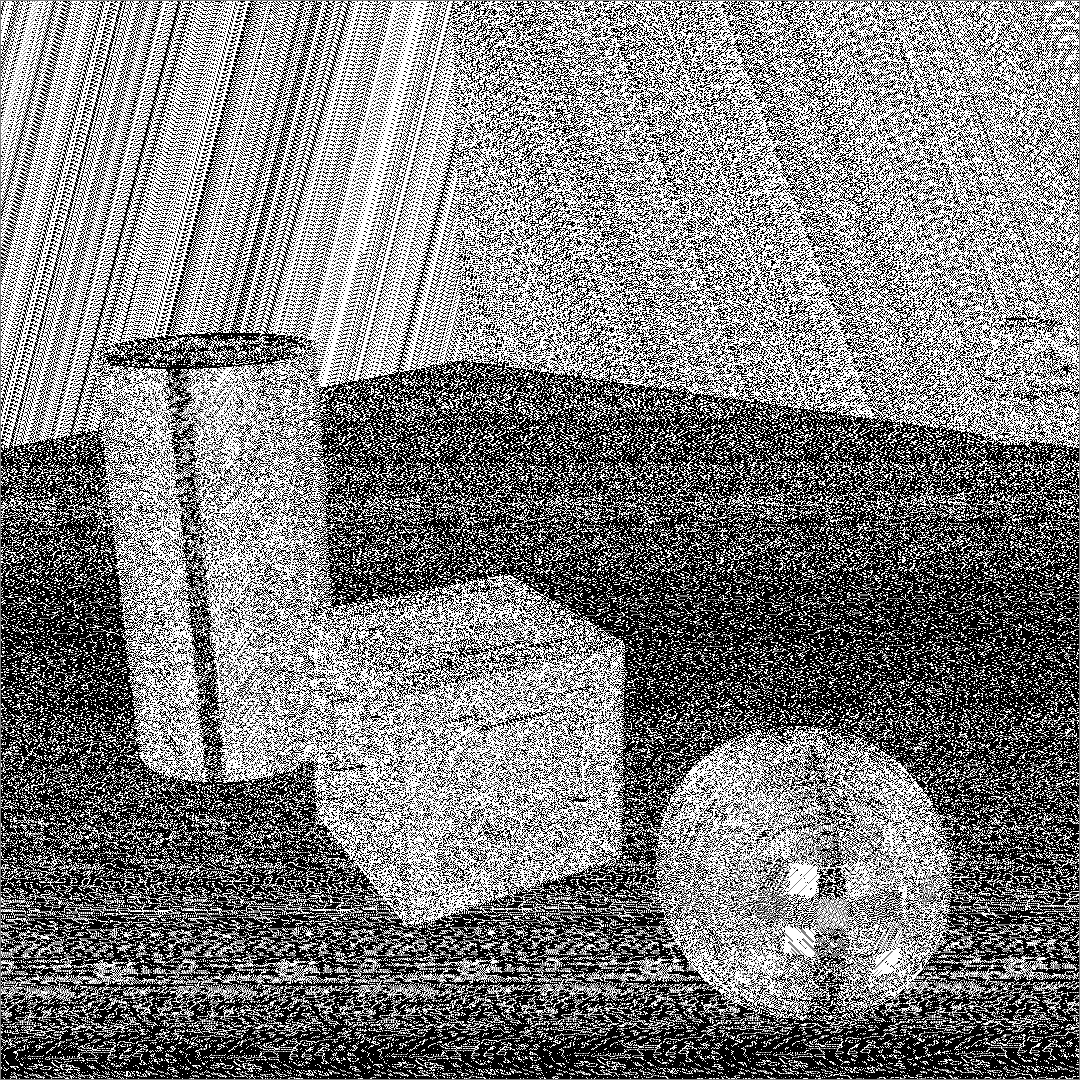
\includegraphics[width=\linewidth]{chapter04/img/gauss-0210.png}
    \end{subfigure}
    \caption[\Gls{gaussian-curvature} in the \emph{Synthetic} scene]{\emph{\Gls{gaussian-curvature} in the Synthetic scene.} The \Gls{gaussian-curvature} feature images for the synthetic scene. The results are not promising either.}\label{fig:gaussian-curvature}
\end{figure}
Computing the curvature for the whole image has the theoretical weakness, that discontinuities at object boundaries are not respected.
The derivatives do not exist at these points for perfect depth sensing.
A mathematically accurate computation requires object identification or meshing of the scene.
Such a requirement seems unreasonable for a foundational processing step in potential real-time use cases.

\subsubsection{\Glspl{flexion-image}}\label{flexion-image-section}

The local shape of an object that is sampled by a depth sensor is characterized by its normalized surface normal.
A surface normal is a vector perpendicular to the surface of the object.
This characterization builds the foundation of the \Gls{flexion-image} and its inspiration, too.

Each measured pixel is backprojected to camera coordinates, scaling the point in spherical coordinates with its measured range, as first step.
Approximating the normal for a measured surface point $\mathbf{P_{i,j}}$ is possible using the cross product of its neighbours connecting vectors.
The point relationship is visualized in Figure~\ref{fig:flexion_normals_plane}.
\begin{figure}[H]
    \begin{subfigure}[t]{0.49\linewidth}
        \centering
        \scalebox{1.0}{%
        

\tikzset{every picture/.style={line width=0.75pt}} %set default line width to 0.75pt        

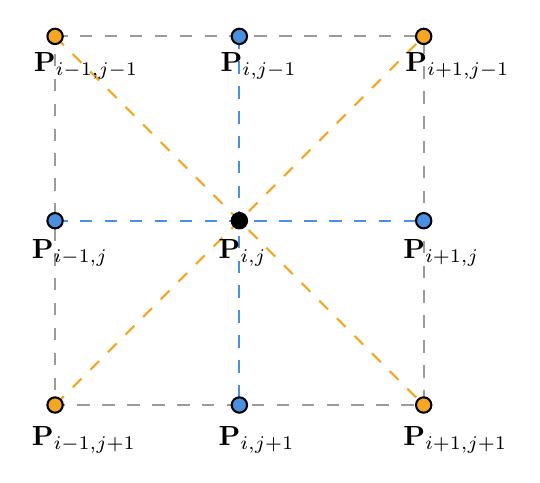
\begin{tikzpicture}[x=0.75pt,y=0.75pt,yscale=-1,xscale=1]
%uncomment if require: \path (0,237); %set diagram left start at 0, and has height of 237

%Shape: Rectangle [id:dp6565487036659107] 
\draw  [color={rgb, 255:red, 155; green, 155; blue, 155 }  ,draw opacity=1 ][dash pattern={on 4.5pt off 4.5pt}] (28.7,13.7) -- (206.3,13.7) -- (206.3,191.3) -- (28.7,191.3) -- cycle ;
%Straight Lines [id:da30195081571029425] 
\draw [color={rgb, 255:red, 74; green, 144; blue, 226 }  ,draw opacity=1 ] [dash pattern={on 4.5pt off 4.5pt}]  (28.7,102.5) -- (206.3,102.5) ;
%Straight Lines [id:da4586174781414081] 
\draw [color={rgb, 255:red, 74; green, 144; blue, 226 }  ,draw opacity=1 ] [dash pattern={on 4.5pt off 4.5pt}]  (117.5,13.7) -- (117.5,191.3) ;
%Straight Lines [id:da7294828306266232] 
\draw [color={rgb, 255:red, 245; green, 166; blue, 35 }  ,draw opacity=1 ] [dash pattern={on 4.5pt off 4.5pt}]  (28.7,13.7) -- (206.3,191.3) ;
%Straight Lines [id:da3243995266948473] 
\draw [color={rgb, 255:red, 245; green, 166; blue, 35 }  ,draw opacity=1 ] [dash pattern={on 4.5pt off 4.5pt}]  (28.7,191.3) -- (206.3,13.7) ;
%Shape: Circle [id:dp5266363779447065] 
\draw  [fill={rgb, 255:red, 245; green, 166; blue, 35 }  ,fill opacity=1 ] (25,13.7) .. controls (25,11.66) and (26.66,10) .. (28.7,10) .. controls (30.74,10) and (32.4,11.66) .. (32.4,13.7) .. controls (32.4,15.74) and (30.74,17.4) .. (28.7,17.4) .. controls (26.66,17.4) and (25,15.74) .. (25,13.7) -- cycle ;
%Shape: Ellipse [id:dp14497174740803043] 
\draw  [fill={rgb, 255:red, 74; green, 144; blue, 226 }  ,fill opacity=1 ] (25,102.5) .. controls (25,100.46) and (26.66,98.8) .. (28.7,98.8) .. controls (30.74,98.8) and (32.4,100.46) .. (32.4,102.5) .. controls (32.4,104.54) and (30.74,106.2) .. (28.7,106.2) .. controls (26.66,106.2) and (25,104.54) .. (25,102.5) -- cycle ;
%Shape: Ellipse [id:dp0427609892023727] 
\draw  [fill={rgb, 255:red, 245; green, 166; blue, 35 }  ,fill opacity=1 ] (25,191.3) .. controls (25,189.26) and (26.66,187.6) .. (28.7,187.6) .. controls (30.74,187.6) and (32.4,189.26) .. (32.4,191.3) .. controls (32.4,193.34) and (30.74,195) .. (28.7,195) .. controls (26.66,195) and (25,193.34) .. (25,191.3) -- cycle ;
%Shape: Ellipse [id:dp2872052196845898] 
\draw  [fill={rgb, 255:red, 74; green, 144; blue, 226 }  ,fill opacity=1 ] (113.8,13.7) .. controls (113.8,11.66) and (115.46,10) .. (117.5,10) .. controls (119.54,10) and (121.2,11.66) .. (121.2,13.7) .. controls (121.2,15.74) and (119.54,17.4) .. (117.5,17.4) .. controls (115.46,17.4) and (113.8,15.74) .. (113.8,13.7) -- cycle ;
%Shape: Circle [id:dp758793708555806] 
\draw  [fill={rgb, 255:red, 0; green, 0; blue, 0 }  ,fill opacity=1 ] (113.8,102.5) .. controls (113.8,100.46) and (115.46,98.8) .. (117.5,98.8) .. controls (119.54,98.8) and (121.2,100.46) .. (121.2,102.5) .. controls (121.2,104.54) and (119.54,106.2) .. (117.5,106.2) .. controls (115.46,106.2) and (113.8,104.54) .. (113.8,102.5) -- cycle ;
%Shape: Circle [id:dp477059334030714] 
\draw  [fill={rgb, 255:red, 74; green, 144; blue, 226 }  ,fill opacity=1 ] (113.8,191.3) .. controls (113.8,189.26) and (115.46,187.6) .. (117.5,187.6) .. controls (119.54,187.6) and (121.2,189.26) .. (121.2,191.3) .. controls (121.2,193.34) and (119.54,195) .. (117.5,195) .. controls (115.46,195) and (113.8,193.34) .. (113.8,191.3) -- cycle ;
%Shape: Ellipse [id:dp13207731000753575] 
\draw  [fill={rgb, 255:red, 245; green, 166; blue, 35 }  ,fill opacity=1 ] (202.6,13.7) .. controls (202.6,11.66) and (204.26,10) .. (206.3,10) .. controls (208.34,10) and (210,11.66) .. (210,13.7) .. controls (210,15.74) and (208.34,17.4) .. (206.3,17.4) .. controls (204.26,17.4) and (202.6,15.74) .. (202.6,13.7) -- cycle ;
%Shape: Circle [id:dp8288145253462365] 
\draw  [fill={rgb, 255:red, 74; green, 144; blue, 226 }  ,fill opacity=1 ] (202.6,102.5) .. controls (202.6,100.46) and (204.26,98.8) .. (206.3,98.8) .. controls (208.34,98.8) and (210,100.46) .. (210,102.5) .. controls (210,104.54) and (208.34,106.2) .. (206.3,106.2) .. controls (204.26,106.2) and (202.6,104.54) .. (202.6,102.5) -- cycle ;
%Shape: Circle [id:dp9160642610677009] 
\draw  [fill={rgb, 255:red, 245; green, 166; blue, 35 }  ,fill opacity=1 ] (202.6,191.3) .. controls (202.6,189.26) and (204.26,187.6) .. (206.3,187.6) .. controls (208.34,187.6) and (210,189.26) .. (210,191.3) .. controls (210,193.34) and (208.34,195) .. (206.3,195) .. controls (204.26,195) and (202.6,193.34) .. (202.6,191.3) -- cycle ;

% Text Node
\draw (106,110) node [anchor=north west][inner sep=0.75pt]   [align=left] {$\displaystyle \mathbf{P}_{i,j}$};
% Text Node
\draw (195,110) node [anchor=north west][inner sep=0.75pt]   [align=left] {$\displaystyle \mathbf{P}_{i+1,j}$};
% Text Node
\draw (16,110) node [anchor=north west][inner sep=0.75pt]   [align=left] {$\displaystyle \mathbf{P}_{i-1,j}$};
% Text Node
\draw (107,20) node [anchor=north west][inner sep=0.75pt]   [align=left] {$\displaystyle \mathbf{P}_{i,j-1}$};
% Text Node
\draw (196,20) node [anchor=north west][inner sep=0.75pt]   [align=left] {$\displaystyle \mathbf{P}_{i+1,j-1}$};
% Text Node
\draw (17,20) node [anchor=north west][inner sep=0.75pt]   [align=left] {$\displaystyle \mathbf{P}_{i-1,j-1}$};
% Text Node
\draw (106,200) node [anchor=north west][inner sep=0.75pt]   [align=left] {$\displaystyle \mathbf{P}_{i,j+1}$};
% Text Node
\draw (195,200) node [anchor=north west][inner sep=0.75pt]   [align=left] {$\displaystyle \mathbf{P}_{i+1,j+1}$};
% Text Node
\draw (16,200) node [anchor=north west][inner sep=0.75pt]   [align=left] {$\displaystyle \mathbf{P}_{i-1,j+1}$};


\end{tikzpicture}


        }
        \caption{The normals for a point $\mathbf{P_{i,j}}$ can be estimated its diagonal or horizontal and vertical neighbours.}\label{fig:flexion_normals_plane}
    \end{subfigure}
    \begin{subfigure}[t]{0.49\linewidth}
        \centering
        \scalebox{1.0}{%
        \begin{tikzpicture}
    \node[anchor=south west,inner sep=0] (image) at (4.0,0) {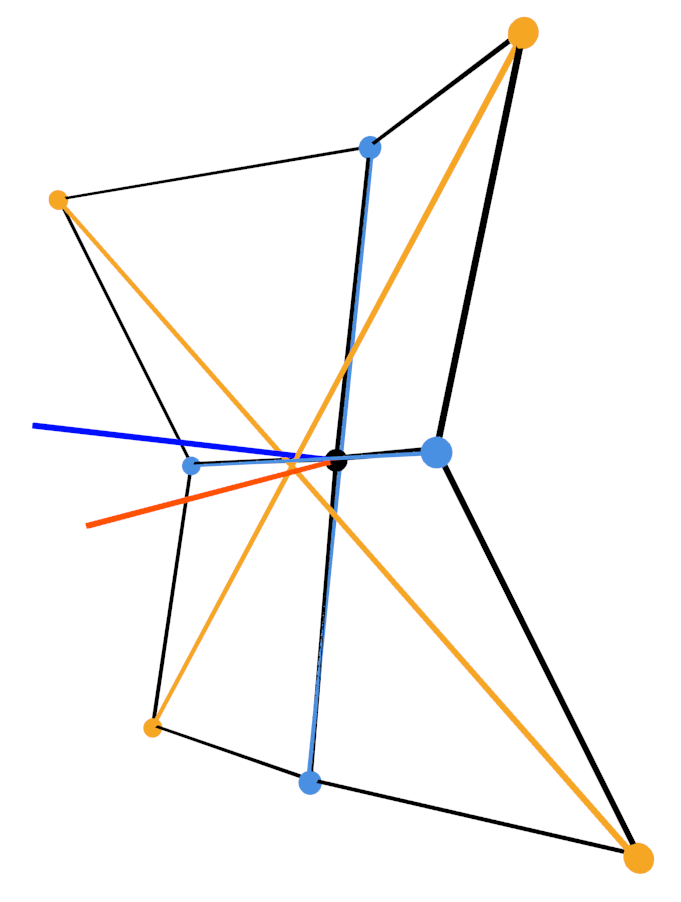
\includegraphics[width=0.6\textwidth]{chapter04/img/flexion-model-2-clipped.png}};
    \node at (4.4, 5.1) {$\mathbf{P_{i-1,j-1}}$};
    \node at (6.2, 5.5) {$\mathbf{P_{i,j-1}}$};
    \node at (8.5, 5.8) {$\mathbf{P_{i+1,j-1}}$};

    \node at (4.7, 2.9) {\scalebox{0.9}{$\mathbf{P_{i-1,j}}$}};
    \node at (6.2, 2.5) {$\mathbf{P_{i,j}}$};
    \node at (7.7, 3.0) {$\mathbf{P_{i+1,j}}$};

    \node at (5.0, 0.9) {$\mathbf{P_{i-1,j+1}}$};
    \node at (6.3, 0.4) {$\mathbf{P_{i,j+1}}$};
    \node at (9.2, 0.3) {$\mathbf{P_{i+1,j+1}}$};

    \node [plotdarkblue] at (4.6, 3.5) {$\vec{n_1}$};
    \node [plotdarkorange] at (4.8, 2.3) {$\vec{n_2}$};
\end{tikzpicture}

        }
        \caption{The estimated normals span an angle depending on the local shape of the surface measured by the depth sensors.}\label{fig:flexion_space}
    \end{subfigure}
    \caption[Schematic representation of the \gls{flexion-image} calculation]{\emph{Schematic representation of the \gls{flexion-image} calculation.} This figure demonstrates how flexed surfaces have different normals for diagonal and non-diagonal estimation. This difference is utilized as measure for flexion.}%
    \label{fig:flexion-image-scetched}
\end{figure}
Using the diagonal and vertical neighbouring points (blue) results a different normal than the diagonal neighbours (orange).
As Figure~\ref{fig:flexion_space} demonstrates, both normals span an angle.
\begin{equation}
\begin{aligned}
    \vec{n_1} &= \frac{\vec{P_{i,j-1}} - \vec{P_{i,j+1}}}{\lnorm{\vec{P_{i,j-1}} - \vec{P_{i,j+1}}}}
                \times \frac{\vec{P_{i-1,j}} - \vec{P_{i+1,j}}}{\lnorm{\vec{P_{i-1,j}} - \vec{P_{i+1,j}}}} \\
    \vec{n_2} &= \frac{\vec{P_{i-1,j-1}} - \vec{P_{i+1,j+1}}}{\lnorm{\vec{P_{i-1,j-1}} - \vec{P_{i+1,j+1}}}}
                \times \frac{\vec{P_{i-1,j+1}} - \vec{P_{i+1,j-1}}}{\lnorm{\vec{P_{i-1,j+1}} - \vec{P_{i+1,j-1}}}}
    \label{eq:flexion_normals}
\end{aligned}
\end{equation}
Note, that both normals $\vec{n_1}$ and $\vec{n_2}$ are not unit length, but only the direction vector between the neighbouring points of $\mathbf{P_{i,j}}$.
Finally, the Flexion $\mathcal{F}$ of point $\mathbf{P_{i,j}}$ is defined as
\begin{align}
    \mathcal{F} &= \abs{\vec{n_1} \cdotp \vec{n_2}}
\end{align}
Because $\lnorm{\vec{n_1}},\lnorm{\vec{n_2}} \in [0,1]$ the value of is bound to $\mathcal{F} \in [0, 1]$.
Creating the final image requires a linear scaling to the desired output image depth using Equation~\ref{eq:linear_scaling}.

Figure~\ref{fig:flexion_images} visualizes the \Gls{flexion-image} for the same camera positions as for the other feature images.
\begin{figure}[H]
    \begin{subfigure}[t]{0.32\textwidth}
        
\includegraphics[width=\linewidth]{chapter04/img/flexion-0001.png}
    \end{subfigure}
    \begin{subfigure}[t]{0.32\textwidth}
        
\includegraphics[width=\linewidth]{chapter04/img/flexion-0030.png}
    \end{subfigure}
    \begin{subfigure}[t]{0.32\textwidth}
        
\includegraphics[width=\linewidth]{chapter04/img/flexion-0210.png}
    \end{subfigure}
    \caption[Characterstic look of a \gls{flexion-image}]{\emph{Characterstic look of a \gls{flexion-image}.} These figures demonstrate the characteristical look of the \Glspl{flexion-image}. Its appearence is very plastic and the shading effects give a good feel for depth. The conversion is rotation invariant.}\label{fig:flexion_images}
\end{figure}

\subsubsection*{Characteristics}

The \gls{flexion-image} is rotation invariant.
Rotation of either an object or the camera does not change the difference between the two normal approximations.
A flat surface has an almost constant shading, because the normal approximation results in the same vector directions.
Flat surfaces not perpendicular to the camera plane have non-constant shading with the brightness reduced the further the surface patch is appart from the camera center.
This effect is caused by the perspective transformation.
The length of the normal vectors reduces with the distance to the camera, because the diagonals gets smaller, as Figure~\ref{fig:flexion_angle_decrease} demonstrates.
\begin{figure}[H]
    

\tikzset{every picture/.style={line width=0.75pt}} %set default line width to 0.75pt        

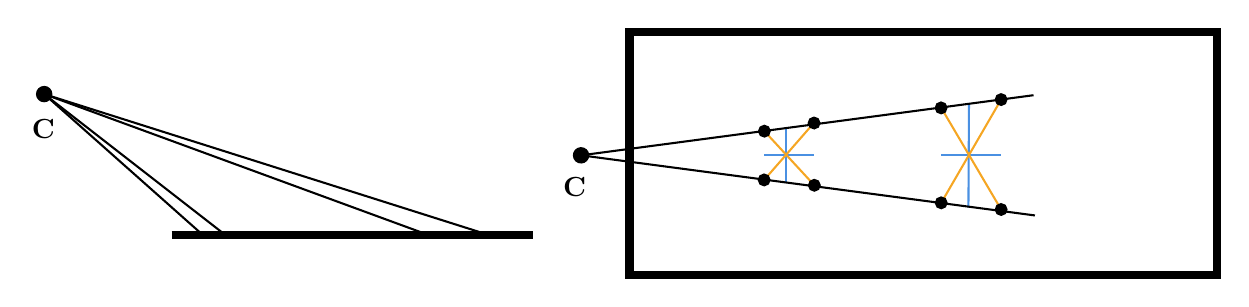
\begin{tikzpicture}[x=0.75pt,y=0.75pt,yscale=-1,xscale=1]
%uncomment if require: \path (0,142); %set diagram left start at 0, and has height of 142

%Straight Lines [id:da6840514143989631] 
\draw [color={rgb, 255:red, 74; green, 144; blue, 226 }  ,draw opacity=1 ]   (366.4,69.04) -- (390.44,69.04) ;
%Straight Lines [id:da9689027017272559] 
\draw [color={rgb, 255:red, 74; green, 144; blue, 226 }  ,draw opacity=1 ]   (377.02,82.13) -- (377.02,55.88) ;
%Straight Lines [id:da8683032061954556] 
\draw [color={rgb, 255:red, 74; green, 144; blue, 226 }  ,draw opacity=1 ]   (451.65,69.04) -- (480.52,69.04) ;
%Straight Lines [id:da6934594327602702] 
\draw [color={rgb, 255:red, 74; green, 144; blue, 226 }  ,draw opacity=1 ]   (464.75,94.04) -- (465.02,44.04) ;
%Straight Lines [id:da7261021710957941] 
\draw [color={rgb, 255:red, 245; green, 166; blue, 35 }  ,draw opacity=1 ]   (480.5,42.14) -- (451.64,91.89) ;
%Straight Lines [id:da37992799055918147] 
\draw [color={rgb, 255:red, 245; green, 166; blue, 35 }  ,draw opacity=1 ]   (451.58,46) -- (480.5,95.1) ;
%Straight Lines [id:da15457235634391941] 
\draw [color={rgb, 255:red, 245; green, 166; blue, 35 }  ,draw opacity=1 ]   (389.38,54.43) -- (366.33,80.86) ;
%Straight Lines [id:da05878950535382432] 
\draw [color={rgb, 255:red, 245; green, 166; blue, 35 }  ,draw opacity=1 ]   (366.45,57.36) -- (390.5,83.43) ;
%Straight Lines [id:da045550454885305736] 
\draw [line width=3]    (80.9,107.5) -- (254.9,107.5) ;
%Shape: Circle [id:dp8549507101465224] 
\draw  [fill={rgb, 255:red, 0; green, 0; blue, 0 }  ,fill opacity=1 ] (16,39.5) .. controls (16,37.59) and (17.54,36.05) .. (19.45,36.05) .. controls (21.36,36.05) and (22.9,37.59) .. (22.9,39.5) .. controls (22.9,41.41) and (21.36,42.95) .. (19.45,42.95) .. controls (17.54,42.95) and (16,41.41) .. (16,39.5) -- cycle ;
%Straight Lines [id:da09684243305909856] 
\draw    (19.45,39.5) -- (94.9,106.5) ;
%Straight Lines [id:da4476141598512392] 
\draw    (19.45,39.5) -- (106.9,107.5) ;
%Straight Lines [id:da5555101325179832] 
\draw    (19.45,39.5) -- (204.9,107.5) ;
%Straight Lines [id:da06573307117836547] 
\draw    (19.45,39.5) -- (230.9,106.5) ;
%Shape: Circle [id:dp3195203497272404] 
\draw  [fill={rgb, 255:red, 0; green, 0; blue, 0 }  ,fill opacity=1 ] (274.67,69.08) .. controls (274.62,67.18) and (276.13,65.6) .. (278.04,65.55) .. controls (279.94,65.51) and (281.52,67.02) .. (281.57,68.92) .. controls (281.61,70.83) and (280.1,72.41) .. (278.2,72.45) .. controls (276.29,72.49) and (274.71,70.99) .. (274.67,69.08) -- cycle ;
%Straight Lines [id:da25083036265050096] 
\draw    (278.12,69) -- (496.79,97.97) ;
%Straight Lines [id:da6083860800665152] 
\draw    (278.12,69) -- (496.1,40.04) ;
%Shape: Rectangle [id:dp031034421219254926] 
\draw  [line width=3]  (301.4,9.5) -- (584.4,9.5) -- (584.4,126.5) -- (301.4,126.5) -- cycle ;
%Shape: Circle [id:dp2988386895287467] 
\draw  [fill={rgb, 255:red, 0; green, 0; blue, 0 }  ,fill opacity=1 ] (363.85,57.42) .. controls (363.81,55.99) and (364.95,54.8) .. (366.39,54.76) .. controls (367.82,54.73) and (369.01,55.87) .. (369.05,57.3) .. controls (369.08,58.74) and (367.94,59.93) .. (366.51,59.96) .. controls (365.07,60) and (363.88,58.86) .. (363.85,57.42) -- cycle ;
%Shape: Circle [id:dp49087747494377276] 
\draw  [fill={rgb, 255:red, 0; green, 0; blue, 0 }  ,fill opacity=1 ] (363.73,80.92) .. controls (363.69,79.48) and (364.83,78.29) .. (366.27,78.26) .. controls (367.7,78.23) and (368.89,79.36) .. (368.93,80.8) .. controls (368.96,82.23) and (367.82,83.42) .. (366.39,83.46) .. controls (364.95,83.49) and (363.76,82.35) .. (363.73,80.92) -- cycle ;
%Shape: Circle [id:dp3291682457892863] 
\draw  [fill={rgb, 255:red, 0; green, 0; blue, 0 }  ,fill opacity=1 ] (387.79,53.49) .. controls (387.75,52.06) and (388.89,50.87) .. (390.32,50.84) .. controls (391.76,50.8) and (392.95,51.94) .. (392.98,53.37) .. controls (393.02,54.81) and (391.88,56) .. (390.44,56.03) .. controls (389.01,56.07) and (387.82,54.93) .. (387.79,53.49) -- cycle ;
%Shape: Circle [id:dp598750640317177] 
\draw  [fill={rgb, 255:red, 0; green, 0; blue, 0 }  ,fill opacity=1 ] (387.91,83.49) .. controls (387.87,82.05) and (389.01,80.86) .. (390.44,80.83) .. controls (391.88,80.79) and (393.07,81.93) .. (393.1,83.37) .. controls (393.14,84.8) and (392,85.99) .. (390.56,86.03) .. controls (389.13,86.06) and (387.94,84.92) .. (387.91,83.49) -- cycle ;
%Shape: Circle [id:dp3156912690396848] 
\draw  [fill={rgb, 255:red, 0; green, 0; blue, 0 }  ,fill opacity=1 ] (449.04,91.95) .. controls (449.01,90.51) and (450.14,89.32) .. (451.58,89.29) .. controls (453.02,89.26) and (454.21,90.39) .. (454.24,91.83) .. controls (454.27,93.26) and (453.13,94.45) .. (451.7,94.49) .. controls (450.26,94.52) and (449.07,93.38) .. (449.04,91.95) -- cycle ;
%Shape: Circle [id:dp0381257221295519] 
\draw  [fill={rgb, 255:red, 0; green, 0; blue, 0 }  ,fill opacity=1 ] (448.99,46.21) .. controls (448.95,44.77) and (450.09,43.58) .. (451.53,43.55) .. controls (452.96,43.52) and (454.15,44.65) .. (454.18,46.09) .. controls (454.22,47.53) and (453.08,48.72) .. (451.65,48.75) .. controls (450.21,48.78) and (449.02,47.65) .. (448.99,46.21) -- cycle ;
%Shape: Circle [id:dp4047969379608699] 
\draw  [fill={rgb, 255:red, 0; green, 0; blue, 0 }  ,fill opacity=1 ] (477.91,42.2) .. controls (477.87,40.76) and (479.01,39.57) .. (480.44,39.54) .. controls (481.88,39.51) and (483.07,40.64) .. (483.1,42.08) .. controls (483.14,43.51) and (482,44.7) .. (480.56,44.74) .. controls (479.13,44.77) and (477.94,43.63) .. (477.91,42.2) -- cycle ;
%Shape: Circle [id:dp5781527725767942] 
\draw  [fill={rgb, 255:red, 0; green, 0; blue, 0 }  ,fill opacity=1 ] (477.91,95.16) .. controls (477.87,93.72) and (479.01,92.53) .. (480.44,92.5) .. controls (481.88,92.46) and (483.07,93.6) .. (483.1,95.04) .. controls (483.14,96.47) and (482,97.66) .. (480.56,97.69) .. controls (479.13,97.73) and (477.94,96.59) .. (477.91,95.16) -- cycle ;

% Text Node
\draw (12,50.05) node [anchor=north west][inner sep=0.75pt]   [align=left] {$\displaystyle \mathbf{C}$};
% Text Node
\draw (268,78.05) node [anchor=north west][inner sep=0.75pt]   [align=left] {$\displaystyle \mathbf{C}$};


\end{tikzpicture}

    \caption[Explanation of shading effect in \glspl{flexion-image}]{\emph{Explanation of shading effect in \glspl{flexion-image}.} The angle between the diagonals decreases with increasing distance from the camera center. This results in shorter normals.}\label{fig:flexion_angle_decrease}
\end{figure}
The origin is the nature of the cross product is maximal if both vectors are perpendicular.
\begin{equation*}
    \lnorm{\vec{v_1} \times \vec{v_2}} = \lnorm{\vec{v_1}} \lnorm{\vec{v_2}} \sin \angle(\vec{v_1}, \vec{v_2})
\end{equation*}
The lack of normalization in Equation~\ref{eq:flexion_normals} propagates this effect through to the scalar product.
\begin{equation*}
    \vec{v_1} \cdot \vec{v_2} = \lnorm{\vec{v_1}} \lnorm{\vec{v_2}} \cos \angle(\vec{v_1}, \vec{v_2})
\end{equation*}
This shading effect gives the \gls{flexion-image} its plastic look and helps to develop the feeling for the geometric constellations.

\subsubsection{Implementation Details}

All software developed during the thesis, including the analysis and supplementary code, are developed with rigor software engineering methods.
The library components have 100\,\% unit- and integrationtest line coverage.
Each final executable is heavily tested, too.
The overall line coverage for all project code is above $98\%$.
The implementation language is C++-17\cite{c++17} and all library depdencies use at least C++-11\cite{c++11}.
All code obeys to strong typing, design by contract\cite{meyer_ieee1992} and modern idioms of the C++ programming language\cite{stroustrup_cpppl2013}.
To uncover runtime problems potentially present in C++ through raw memory access, the LLVM Address-, Memory-, Thread- and Undefined-Behaviour-Sanitizers\cite{google_sanitizers} are run over all tests.
Additional static analysis is done by clang's thread-safety analysis\cite{clang_thread_safety}, clang static analyzer\cite{clang_static_analyzer} and clang-tidy\cite{babati2017static}.
All detected issues were immediately fixed during development.
The use of continuous integration\cite{fowler_ci2000} for the whole development cycle indicated defects within hours and ensured fast development of code with a low defect rate.

The implementation goal of the developed software is to serve as a correct reference implementation for the proposed feature images.
Therefore, no special action has been taken to improve latency or throughput of the computations.
Only simple measures for speedup, namely exploiting the embarrassingly parallel nature of the processing and compiler optimizations are employed.
Figure~\ref{fig:benchmarks} shows the results of micro benchmarks of the two promising feature images.
\begin{figure}
\centering
    \begin{subfigure}[b]{0.45\linewidth}
        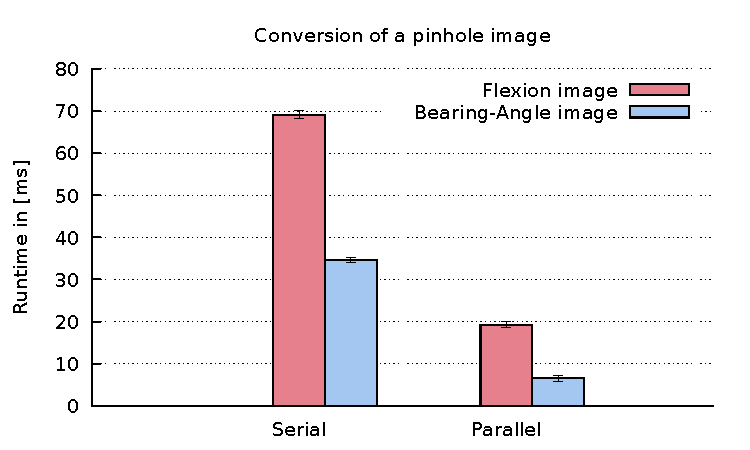
\includegraphics[width=\linewidth]{chapter06/results/benchmarks/pinhole_benchmarks.pdf}
    \end{subfigure}\quad
    \begin{subfigure}[b]{0.45\linewidth}
        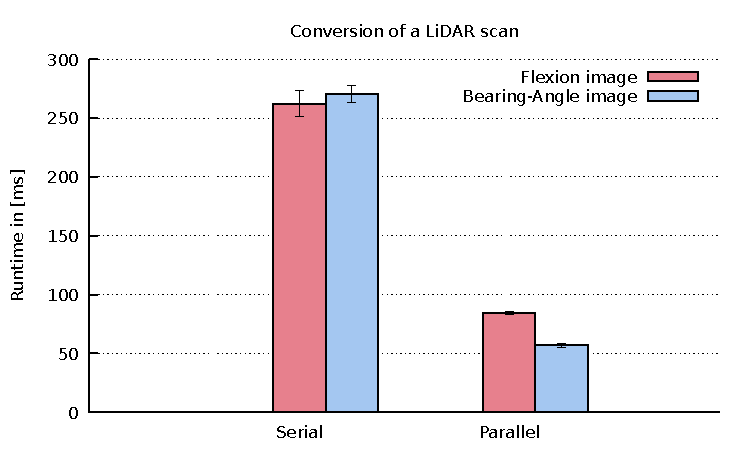
\includegraphics[width=\linewidth]{chapter06/results/benchmarks/laserscan_benchmarks.pdf}
    \end{subfigure}
    \caption[Benchmarks for Flexion and \gls{bearing-angle-image} conversions]{\emph{Benchmarks for Flexion and \gls{bearing-angle-image} conversions.} The benchmarks are run on an Intel i7-8550U with 1.8\,GHz base clock and 4 hyperthreaded cores. Each conversion is repeated 100 times for solid statistical data. The resolution of the pinhole image is 960$\times$540\,px and the \acrshort{LIDAR} scan is 3600$\times$800\,px big. The higher memory consumption of the \acrshort{LIDAR} scan results in a memory bound execution for the single threaded conversion.}\label{fig:benchmarks}
\end{figure}
Each of the feature image conversions is implemented as C++ library code working on OpenCV's\cite{opencv_library} \lstinline[basicstyle=\ttfamily]|cv::Mat| matrix type.
The conversion is generic in the sense, that any camera model implementing the forward and backward projection for pixel coordinates is suitable for the feature image conversion.
This genericity is achieved through the use of templates.
Type requirements are enforced with \lstinline[basicstyle=\ttfamily]|static_assert()| and concept-like\cite{c++concepts} requirement definitions.
One important type requirement ensures consistent use of coordinate systems with a special type that prohibits the code \texttt{\lstinline[language=C++,basicstyle=\footnotesize\ttfamily]|coordinate<float, frame::pixel> px = coordinate<float, frame::image>(0.5F, 0.25F);|} to compile.
All image access operations must adhere to the reference frame annotation and special transformations, like projections, are the only way to switch between coordinate systems.

Multiple library dependencies support the functionality of the project and shall be mentioned without a particular order.
The already mentioned OpenCV\cite{opencv_library} project provides functionality for image handling and processing. 
Required types and functionality for glue-code, parallelization and general programming utilize \emph{cli11}\cite{cli11}, \emph{rang}\cite{rang}, \emph{cpp-taskflow}\cite{Huang2019CppTaskflowFT}, \emph{fmt-lib}\cite{fmtlib}, \emph{GSL}\cite{gsl}, \emph{Eigen3}\cite{eigenweb} and \emph{Boost}\cite{boost}.
Functionality and performance testing are done with \emph{doctest}\cite{doctest} and \emph{libnonius}\cite{libnonius}.
Each used revision is documented in the code repository and differs between versions of the thesis code.

